\documentclass[11pt,a4paper]{article}
\usepackage[utf8]{inputenc}
\usepackage[T1]{fontenc}
\usepackage[margin=2.5cm]{geometry} % Reasonable margins
\usepackage{lmodern} % Modern font
\usepackage{graphicx} % For including images
\usepackage{amsmath} % For math equations
\usepackage{amsfonts} % Math fonts
\usepackage{amssymb} % Math symbols
\usepackage{booktabs} % Better tables
\usepackage{lineno} % For line numbers if needed
\usepackage{setspace} % For line spacing
\usepackage{parskip} % Better paragraph spacing
\usepackage{physics}
\usepackage{enumitem}
\usepackage{float} % For [H] placement specifier
\usepackage[colorlinks=true,urlcolor=blue,linkcolor=blue]{hyperref} % For hyperlinks



%For incerting blocks of code!
\usepackage{listings}
\usepackage{xcolor}

\lstset{
    language=Python,
    basicstyle=\ttfamily\small,
    keywordstyle=\color{blue},
    commentstyle=\color{gray},
    stringstyle=\color{orange},
    showstringspaces=false,
    frame=single,
    breaklines=true
}


% Set line spacing to 1.5
\onehalfspacing

% Title information
%\title{\textbf{Quantum Reservoir Computing}}\\
%\author{Angelos Aslanidis}
\date{\today}

\begin{document}


\begin{titlepage}
    \centering
    
    % University and department
    {\Large\scshape Ludwig-Maximilians-Universität München} \\[0.3cm]
    {\large Faculty of Physics \\ 
    AI in Physics Research Group} \\[1.5cm]
    
    % Horizontal rule with spacing
    \vspace{0.4cm}
    \rule{\textwidth}{1pt} \\[0.4cm]
    
    % Main title (two lines)
    {\fontsize{22}{26}\selectfont\bfseries PP} \\[0.4cm]
    
    \rule{\textwidth}{1pt} \\[1.5cm]
    
    % Authors
    \textbf{Group A} \\[0.3cm]
    \begin{tabular}{c}
        Vyron Arvanitis \\ 
        Emanuele Poggi \\ 
        Paul Hofmann \\ 
        Moritz Heidtmann \\ 
        Angelos Aslanidis
    \end{tabular} \\[2cm]
    
    % Supervisor
    \textbf{Supervisor} \\[0.3cm]
    Nikolai Krug \\[1.5cm]
    
    % Date
    {\large \today}
    
\end{titlepage}




\tableofcontents
\newpage
\section{Introduction}
In this lab course, we work with simulated data from the Belle II 
experiment to develop a fast and efficient simulation pipeline.
The goal is to train and compare machine learning models that can predict 
early in the simulation chain whether an event is likely to survive 
later selection stages. 
This allows us to discard unimportant background events early,
saving computational resources typically spent on full detector simulation 
and reconstruction (processess which are far more comptutaionaly expensive). 
The strategy is illustrated in Fig.~\ref{fig:smart_sim}, 
where a neural network acts as a pre-filter to speed up 
the overall simulation process.
\begin{figure}[h]
    \centering
    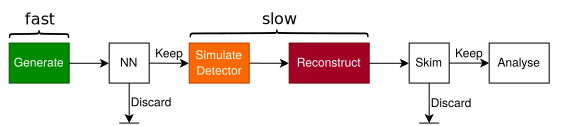
\includegraphics[width=\textwidth]{chapters/introduction/MC_data_flow-keep-discard_NN.png}
\caption{Smart simulation strategy: a neural network filters generated events 
before expensive detector simulation. 
Figure adapted from the official LMU AI Lab repository~\cite{ai-lab-repo}.}
    \label{fig:smart_sim}
\end{figure}

\section{The Belle experiment}

The Belle experiment is a so-called \emph{B-Factory}, 
a type of particle accelerator specifically designed to 
produce large numbers of \emph{B mesons}. 
These factories operate with a center-of-mass energy tuned 
to the \emph{$\Upsilon(4S)$ resonance}, 
a state that decays almost exclusively 
into pairs of $B$ and $\bar{B}$ mesons. 
This production mechanism enables detailed studies 
of $B$ meson decays, allowing physicists to investigate 
phenomena such as \emph{CP violation}, rare decays, 
and physics beyond the Standard Model. 
The Belle~II experiment, located at the \emph{SuperKEKB collider in 
Tsukuba, Japan}, is the successor to the original 
Belle experiment and significantly improves on its 
precision and data collection capabilities.

Unlike proton-proton colliders (such as the LHC), Belle~II uses 
electron-positron ($e^+e^-$) collisions. Electrons and positrons 
are elementary particles with no internal structure, this offers 
several advantages. First, their interactions are much cleaner, and 
the background is easier to interpret—there is a notable absence of 
hadronic activity such as jets. Moreover, the absence of 
internal substructure allows us to precisely know the initial momenta 
of the colliding particles, enabling accurate reconstruction of the 
event kinematics. This precision is crucial for tuning the  
aforementioned center-of-mass energy to specific resonances, 
such as the $\Upsilon(4S)$.

$B$ mesons are unstable particles that decay via the 
weak interaction, and their decays can be classified into 
three categories: hadronic, semileptonic, and rare  decays. 
In \emph{hadronic decays}, the $B$ meson decays into only 
hadrons, such as combinations of kaons ($K$), pions ($\pi$), 
and other mesons. \emph{Semileptonic decays} involve 
both hadrons and leptons, typically resulting in a final 
state containing a charged lepton ($e^\pm$ or $\mu^\pm$), 
a neutrino, and hadrons. \emph{Rare decays} may involve photons,
multiple leptons, or other suppressed processes that are 
especially sensitive to effects beyond the Standard Model.
These decay modes provide a rich ground for studying CP 
violation, flavor physics, and potential new physics.

The Belle~II detector is structured as a layered system of 
subdetectors (like an onion) built around the interaction point.
Closest to the interaction region is the Vertex Detector (VXD), 
composed of the PiXel Detector (PXD) and Silicon 
Vertex Detector (SVD), which provide precise tracking 
information for reconstructing decay vertices. 
Surrounding the VXD is the Central Drift Chamber (CDC), 
responsible for tracking charged particles and measuring 
their momenta and energy loss. 
Particle identification is handled by the Time Of 
Propagation (TOP) detector in the barrel region and the 
Aerogel Ring Imaging Cherenkov (ARICH) detector in the 
forward region.Photons and electrons are measured in the 
Electromagnetic Calorimeter (ECL) via the production of showers,
while muons and long-lived neutral kaons ($K_L^0$) are 
identified in the outermost KLong and Muon (KLM) detector. 
The entire setup is enclosed in a $1.5~T$ magnetic field provided 
by a superconducting solenoid, which not only alligns the beams
but also enables accurate momentum measurements. An overview 
of the collider (figure~\ref{fig:belle-detector-overview} ) and the particles that can be identified in each 
subdetector can be seen in table~\ref{table:belle-subdetectors}


\begin{figure}[h]
    \centering
    \includegraphics[width=0.8\linewidth]{chapters/Belle_experiment/Overview_collider.png}
    \caption{Closeup of the Belle~II detector indicating 
    all the different subdetectors~\cite{belle2-image}.}
    \label{fig:belle-detector-overview}
\end{figure}


\begin{table}[h]
\centering
\begin{tabular}{ll}
\toprule
\textbf{Subdetector} & \textbf{Main Purpose} \\
\midrule
PXD + SVD (VXD) & Track reconstruction near the IP, measures short-lived particles \\
CDC             & Tracking of charged particles \\
TOP / ARICH     & Particle identification (e.g. distinguish $\pi$, $K$, $p$) via Cherenkov radiation \\
ECL             & Detection of electrons and photons (electromagnetic showers) \\
KLM             & $\mu$ identification and detection of $K_L^0$ \\
\bottomrule
\end{tabular}
\caption{Belle~II subdetectors and the particles they primarily detect.}
\label{table:belle-subdetectors}
\end{table}


\subsection{Problem Description}

The Belle~II experiment collects an enormous amount of data,
with its center-of-mass energy tuned to the $\Upsilon(4S)$ resonance 
\emph{corresponding to a center-of-mass energy of $\sqrt{s} = 10.58$~GeV}. 
While these "resonant" events are the primary source 
for $B$ physics, Belle~II also records other types 
of data.

To achieve this center-of-mass energy the two beams colliding have respective
energies of $7\, \text{GeV}$ and $4\, \text{GeV}$. This assymetric beam 
configuration introduces a forward boost to the CoM system, forcing the 
produced $B$ (and $\bar{B}$) mesons to travel measurables distances
in the detector before they decay.

\begin{figure}[h]
    \centering
    \includegraphics[width=0.75\linewidth]{chapters/Belle_experiment/Belle_resonances.png}
    \caption{Cross section of $e^+e^-$ with respect to the center-of-mass energy [GeV] \cite{belle2-Y-resonances}.}
    \label{fig:upsilon-resonances}
\end{figure}

To reduce the data volume and focus on interesting events, 
Belle~II employs a two-level filtering system: 
the Level-1 hardware trigger (TRG) and the High Level Trigger (HLT), 
which together reduce the event rate before data is stored. 
Even after this, the number of events retained is still too large 
for direct analysis, so further selection — known as skimming — is 
performed to extract smaller datasets.

In parallel, Monte Carlo (MC) simulations are used to model the 
detector response and to train and validate analysis strategies.
These simulated events must pass through all stages of detector 
simulation, digitization, reconstruction, and selection, mirroring 
the real data processing pipeline. However,this process is 
computationally expensive, especially when simulating large 
background samples, most of which are eventually discarded by skims.

To address this issue, the goal of this lab course is to
explore a technique known as \emph{Smart Background Simulation}. 
Instead of fully simulating every event, we aim to train a neural 
network that can predict early on whether a given event will survive a 
later skim. This skim selects events in which at least one $B^0$ meson 
can be reconstructed through hadronic decays. 
After building several neural networks we evaluate their performance
on an independent test set and calculate the speedup offered by each network.







\section{Theory}
\subsection{Deep Sets} \label{sec:DeepSet}
In many physical systems, such as collections of particles or events in high-energy physics, the data can be naturally represented as unordered sets. Traditional neural networks, however, are not inherently permutation-invariant. This means that they assume an order in their input. To address this, Deep Sets provide a principled way to process such set-structured data while maintaining invariance to the order of elements. Figure \ref{fig:deepset} visualizes the structure of a Deep Set model. 

\begin{figure}[h]
    \centering
    \includegraphics[width=0.7\linewidth]{chapters/theory/deep_set.png}
    \caption{Schematic illustration of a Deep Set model.}
    \label{fig:deepset}
\end{figure}

A Deep Set model operates by applying a shared function $\phi$ independently to each element in the set. This produces a new set of embeddings, which are then aggregated using a permutation-invariant operation such as sum, mean, or max. The aggregated result is passed through a second function $\rho$, typically implemented as a multilayer perceptron (MLP), to produce the final output:

\begin{equation}
    f(X) = \rho\left( \sum_{x \in X} \phi(x) \right)
\end{equation}

This structure ensures that the model respects the symmetry of sets. The theoretical foundation of Deep Sets is discussed in \cite{zaheer2017deep}, where it is shown that any function on a set that is invariant to permutations can be decomposed in this form.

In our project, we use this architecture to model collections of particles, where the order of particles is physically irrelevant. The Deep Set model thus provides a natural and efficient baseline for learning from such data.

\subsection{Graph Convolutional Neural  Networks} \label{sec:GCN}
In contrast to Deep Set models, which treat the input as an unordered collection, Graph Neural Networks (GNNs) explicitly leverage relational information between data points. This is particularly important in our context, where particles are connected through a decay tree structure that naturally forms a graph. Each node in the graph represents a particle, and edges represent physical relationships (e.g., parent-child connections in the decay chain).

In terms of Deep Sets, graph convolutions can be seen as permutation equivariant operations. As long as the aggregation function (e.g., sum, mean, or max) is symmetric, the update remains invariant to the ordering of neighbors.

\begin{figure}[h]
	\centering
	\includegraphics[width=0.7\linewidth]{chapters/theory/cnn_vs_gcn.jpg}
	\caption{Analogy between CNNs and GCNs. In CNNs, pixels are updated based on spatial neighborhoods; 
    in GCNs, nodes are updated based on graph neighborhoods. \cite{zhihu-figure-qc} }
	\label{fig:gcn}
\end{figure}

Figure \ref{fig:gcn} illustrates the analogy between Convolutional Neural Networks (CNNs) and Graph Convolutional Networks (GCNs). In CNNs, pixels are updated based on their spatial neighborhoods, while in GCNs, nodes are updated based on their graph neighborhoods. This allows GNNs to capture complex relationships and dependencies in the data, making them particularly suitable for tasks involving structured data like particle decays.


\subsection{Multi Layer Perceptron}\label{sec:theory_mlp}
A Multi‐Layer Perceptron (MLP) is the canonical feed‐forward neural network: a sequence of fully‐connected layers interleaved with nonlinear activation functions.  Each layer computes
\[
h^{(\ell)} = \phi\bigl(W^{(\ell)} h^{(\ell-1)} + b^{(\ell)}\bigr),
\]
where \(W^{(\ell)},b^{(\ell)}\) are the layer’s learnable weights and biases, and \(\phi\) is a pointwise nonlinearity such as ReLU. Figure \ref{fig:mlp}  showS the structure of a vanilla MLP.

MLP are universal function approximators: by stacking several layers, an MLP can approximate arbitrarily complex mappings from its fixed‐length input vector to the desired output.


\begin{figure}[h]
	\centering
	\includegraphics[width=0.7\linewidth]{chapters/theory/mlp_1.png}
	\caption{Schematic illustration of a Multi‐Layer Perceptron. \cite{turing} }
	\label{fig:mlp}
\end{figure}

Because an MLP operates on a flat vector of features, it requires a predetermined input size and implicitly assumes an ordering of those inputs.  In tasks where the data are naturally sets or graphs (e.g.\ collections of particles), this fixed‐order assumption provides no mechanism to enforce permutation invariance or to leverage relational structure.  


\subsection{Transformer} \label{sec:Transformer}

The Transformer architecture was introduced by Vaswani 
\cite{DBLP:journals/corr/VaswaniSPUJGKP17}.
The key ingredient in the success of the Transformer is the \emph{self-attention} mechanism, 
which enables the model to 
capture long-range dependencies between elements of the input. 

The encoder takes the input sequence (in our case, the set of particles 
in an event),  
maps  tokens such as PDG identifiers to dense embedding vectors,  
adds positional encodings, and processes them through multiple layers 
of multi-head self-attention and feedforward sublayers. 
Each encoder layer contains connections and layer normalization,  
allowing information to propagate effectively through the network.
In our architecture, only the encoder component of the Transformer is used,  
as our task is classification rather than sequence generation.


The outputs of the decoder are generated by attending both 
to the encoder outputs and to its own previously generated tokens.  
It introduces a \emph{masked} self-attention mechanism to prevent the model 
from attending to future positions in the output sequence.  
Since our problem does not involve generating sequences, 
the decoder component is omitted in our implementation.  


The attention mechanism computes a weighted sum of vectors,  
where the weights are determined by the similarity between a 
query vector and a set of key vectors.  
In the multi-head self-attention setting, several independent attention “heads” 
are computed in parallel, allowing the model to focus on different types 
of relationships simultaneously.  
Self-attention enables each particle to directly incorporate information from 
all others in the event.
The afformentioned property makes the transformer architecture highly suitable for
particle physics tasks!

\begin{figure}[H]
    \centering
    \includegraphics[width=0.7\linewidth]{chapters/theory/Transformer_architecture.png}
    \caption{Transformer-model architecture \cite{DBLP:journals/corr/VaswaniSPUJGKP17}}
    \label{fig:Transformer_architecture}
\end{figure}

\section{Methodology}

To identify the optimal model architecture, each group member conducted 
small-scale investigations targeting specific aspects of the model design. 
These investigations included the following:

\begin{itemize}
    \item Does it help to increase the number of linear layes?
    \item Which sequence of GCN and Linear layers works best?
    \item Is it possible to use a standard MLP as well? If yes how?
    \item How important is the masking in this case?
    \item Methods to combat overfitting
    \item Do we need to transform the values for the particle features?
    \item Are there any redundant features in the dataset that could be removed?
    \item Could one make use of some (approximate) symmetries in the data? 
    \item Ideas for different model architectures
\end{itemize}


\subsection{The Dataset}

The dataset of the experiment consists of simulated particle collision events, with 
each event containing multiple decay particles. These events contain a variable number of final state and intermediate particles. Hence, they can be structured as a graph, where each particle is a node and the edges represent the relationships between particles (e.g., parent-child relationships in decays). The graph can be seen in figure \ref{fig:graph_example}.

\begin{figure}[H]
 \centering
    \includegraphics[width=0.75\textwidth]{chapters/methodology/particle_graph.png}
    \caption{Example of a particle decay graph. The nodes represent particles, 
    and the edges represent the decay relationships between them.}
    \label{fig:graph_example}
\end{figure}

Each particle is described by a fixed number of features, which include:

\begin{itemize}
    \item \texttt{prodTime} — the production time of the particle,
    \item \texttt{energy} — the energy of the particle,
    \item \texttt{x}, \texttt{y}, \texttt{z} — the spatial coordinates of the particle at production,
    \item \texttt{px}, \texttt{py}, \texttt{pz} — the momentum components of the particle,
    \item \texttt{pdg} — the PDG identifier of the particle, indicating its type,
    \item \texttt{index}, \texttt{mother\_index} — the particle’s index and the index of its mother particle (if any).
    \item \texttt{label} — this indicates weather or not the particle has passed the downstream event selection or not, it takes binary values 0 or 1
\end{itemize}

Each event is represented as a tensor of shape \texttt{(num\_particles, num\_features)}. 
Since the number of particles can vary between events, padding is applied to ensure consistent input dimensions across batches. These padded values are properly masked during training to prevent them from affecting the model.

\subsection{Transforming the feature values} \label{sec:Nomralize features}

For this investigation, we used our best model obtained after the first 
lab day — that is \textbf{CombinedModel with GCN} model — and focused on normalizing
the inputs. The normalization was done according to the following function


\begin{lstlisting}
def normalize_inputs(inputs):
    x = inputs["feat"] # with "feat" we mean the position, momentum vectors, the production time and the Energy
    # x.shape = (batch_size, num_particles, num_features)
    mean = x.mean(dim=(0,1), keepdim=True)  # Collapse batch and particle dimensions; end up with (num_features) -> one mean per feature!
    std = x.std(dim=(0,1), keepdim=True) + 1e-8  # avoid divide-by-zero
    x_norm = (x - mean) / std
    return {**inputs, "feat": x_norm}
\end{lstlisting}

Essentially, we subtracted the mean and divided by the standard deviation of each feature, calculated across 
both the batch and particle dimensions. 

\subsection{Unecessary Features}

To investigate whether or not some features are unnecessary in our analysis,
we used again the same model (\textbf{CombinedModel with GCN}) and evaluated it,
subtracting features via physical arguments. We performed six tests. 

First of all, we removed the momentum vector ($\vec{p}$). The argument for this was that 
the energy and momenta of a particle are associated with the well-known relationship:
\[
E^2 = p^2 + m^2
\]
so, in principle, the model could reconstruct the momenta from the energy (or vice versa), assuming the mass is constant or implicitly learned.

For the same reason mentioned above, we explored removing the energy of the particles.

Afterwards, we removed the position vectors $x$, $y$, and $z$. 
This started as a simple test, however the following argument was made: 
in our problem, there exists a cylindrical symmetry — the $x$ and $y$ axes can be arbitrarily chosen (as the beams are considered to be colliding along the $z$ axis). Therefore, we considered removing only the $x$ and $y$ coordinates. 

However, after consideration we came to the conclusion that this is 
physically wrong because removing both $x$ and $y$ would eliminate any 
information about the transverse plane. Therefore, we opted to remove only the 
$x$ position coordinate, as a compromise to test sensitivity to symmetry 
arguments.

In the end, we removed the \texttt{prodTime} feature just for further 
analysis, since its physical importance was unclear and we wanted to check 
if it had any significant impact on performance.

\begin{figure}[H]
 \centering
    \includegraphics[width=0.75\textwidth]{chapters/methodology/feature_importance_comparison.png}
    \caption{Validation accuracy and loss for different experiments. 
    The horizontal dashed lines indicate the best performance 
    achieved with the baseline model. Note: the \textbf{reversed} 
    model refers to the configuration where the GCN 
    and DeepSet layers were swapped.}
    \label{fig:Feature_importance}
\end{figure}

From figure \ref{fig:Feature_importance} it is evident that no significant 
improvement in model performance was observed when removing features. In all 
cases, the validation accuracy and loss remained close to the baseline values. The only 
slight performance gain was observed when applying normalization to the input 
features, confirming its importance as a preprocessing step.
    

\subsection{Speedup}

To evaluate the efficiency of using a NN as a filter before detector simulation, we define the speedup as the ratio of time needed to process events \emph{without} and \emph{with} the NN, for the same number of positively selected (skimmed) events.

Let:
\begin{itemize}
    \item \( t_g \): time for event generation
    \item \( t_s \): time for detector simulation and reconstruction
    \item \( r = 0.05 \): fraction of events passing the original skim (without NN)
    \item \( f_1 \): true positive rate (TPR)
    \item \( f_0 \): false positive rate (FPR)
    \item \( X \): number of events generated
\end{itemize}

Further, we define:
\begin{align*}
    X_i &= r \cdot X \quad \text{(number of events passing skim)} \\
    X_i &= f_1 \cdot X' \quad \text{(true positives from NN)} \\
    \Rightarrow X' &= \frac{r}{f_1} \cdot X \quad \text{(number of events to be generated with NN)} \\
    P &= f_1 \cdot X' + f_0 \cdot (1 - r) \cdot X \quad \text{(events passing NN)} \\
\end{align*}

The speedup is the ratio of total time without and with NN:
\[
\text{Speedup} = \frac{X \cdot (t_g + t_s)}{X' \cdot t_g + P \cdot t_s}
\]

Substituting \( X' \) and \( P \) into the equation:
\[
\text{Speedup} = \frac{f_1 \cdot (t_g + t_s)}{t_g + t_s \cdot \left( f_1 + f_0 \cdot \frac{1 - r}{r} \right)}
\]

Finally, assuming \( t_s = 100 \cdot t_g \), we simplify to:
\[
\text{Speedup} = \frac{101 \cdot f_1}{1 + 100 \cdot \left( f_1 + f_0 \cdot \left( \frac{1 - r}{r} \right) \right)}
\]

\subsection{Models architecture}

From our comulative research we came to the conclusion that the following
are the best models, we mention also more simplistic models as it is 
interesting to see the impact that additional layers or methods of 
regularization have on the performance.

\subsubsection*{DeepSet Model} \label{model:DeepSet}

This model follows the Deep Sets framework (as mentioned in \ref{sec:DeepSet}), 
where the same transformation is applied independently to each element of the input set before aggregation.

\paragraph{Architecture.} 
The model takes as input a batch of events, where each event consists of a 
list of particles. Each particle is represented by a feature vector.
The architecture consists of the following components:

\begin{itemize}
    \item Linear layer with Relu activation function
    \item A masking layer with averaging over the masked events or averaging if no masks exists
    \item Linear layer with Relu activation function
    \item Output layer (a single neuron)

\end{itemize}

\subsubsection*{Combined Model} \label{model:CombinedModel}

This model extends the deepset architecture by introducing PDG code to each particles
afterwards mapped to an embedding vector. The embedding vectors are added to the original 
particle feature before being processed by the rest of the network

\paragraph{Architecture.}
The model processes a batch of events, where each particle is represented by both a feature vector and a PDG code. 
The architecture consists of the following components:

\begin{itemize}
    \item Embedding layer that maps each PDG code to a vector.
    \item Concatenation of the PDG embedding with the original particle features.
    \item Linear layer with ReLU activation function.
    \item A masking layer with averaging over the masked events or simple averaging if no mask is used.
    \item Linear layer with ReLU activation function.
    \item Output layer (a single neuron).
\end{itemize}

\subsubsection*{DeepSet with GCN} \label{model:DeepSet_wGCN}

This model combines a Graph Convolutional Network (GCN) layer with the Deep Set architecture.
The GCN captures local structure between particles as defined by an adjacency matrix (typically based on mother-daughter relations), 

\paragraph{Architecture.}
The input consists of a set of particles (each with a feature vector) and a corresponding adjacency matrix encoding  connections between particles. 
The architecture includes the following components:

\begin{itemize}
    \item A GCN layer that applies a linear transformation to each particle this is done by multiplying the normalized adjacency matrix with a linear layer
    \item A DeepSet layer that aggregates the GCN output using a masked mean over particles, followed by a linear transformation with ReLU activation.
    \item An output layer (a single neuron) that produces the final prediction.
\end{itemize}

\subsubsection*{Combined Deepset with GCN} \label{model:CombinedModel_wGCN}
This model extends the DeepSet with GCN architecture by introducing a  PDG code to each 
particles afterwards mapped to an embedding vector

\paragraph{Architecture.}
The input consists of particle features, PDG codes, and an adjacency matrix. 
The architecture includes the following components:

\begin{itemize}
    \item An embedding layer that maps each PDG code to a vector.
    \item A droupout layer with a droupout rate of $0.3$.
    \item Concatenation of the PDG embedding with the original particle features and the normalized adjacency matrix.
    \item A GCN layer applied to the concatenated inputs.
    \item A batch normalization layer 
    \item A dropout layer with a droupout rate of $0.3$
    \item A Deep Set layer.
    \item An output layer (a single neuron) that produces the final prediction.
\end{itemize}


\subsubsection*{Combined Deepset with GCN Normalized} \label{model:CombinedModel_wGCN_Normalized}
This model extends the Combined Deepset with GCN architecture (model \ref{model:CombinedModel_wGCN})
by introducing a normalization of the inputs according to section \ref{sec:Nomralize features}.

\paragraph{Architecture.}
The architecture is the same as in the case of \ref{model:CombinedModel_wGCN}
with an additional normalization layer.



\subsubsection*{Transformer} \label{model:Transformer}



\section{Models Used in the End}
Based on our comulative research, we identified the following models as the most promising. We also include simpler baseline architectures, as they help illustrate the impact of additional layers and regularization techniques on model performace. 

\subsection{General setup}
All models described below take at least the following arguments:
\begin{itemize}
    \item \texttt{num\_features} (int): Number of input features
    \item \texttt{units} (int): Number of hidden units
\end{itemize}

To describe the shapes of the model layers, we adopt the following notation:
\begin{itemize}
    \item $B$: Batch size
    \item $N$: Number of particles per event
    \item $f$: Number of input features
    \item $u$: Number of hidden units
\end{itemize}

The input to every model is given by $B$ batches, each containing $N$ particles, each having $f$ features. The input shape is therefore $[B,N,f]$.
Any deviation will be further specified for each model individually.

\subsection{DeepSet Model} \label{model:DeepSet}

This model follows the Deep Sets framework (as introduced in Section \ref{sec:DeepSet}), 
in which the same transformation is applied independently to each element of the input set, followed by a permutation-invariant aggregation. All other models are built upon this base architecture. 

The architecture of the model is summarized in table \ref{tab:deepset_arc}.
\begin{table}[h]
    \caption{DeepSet Model Architecture}
    \label{tab:deepset_arc}
    \centering
    \begin{tabular}{l|l|c|c}
        \hline
        Layer \# & Description & Output shape & Parameters \\
        \hline 
        1 & Linear + ReLU (shared across particles) & $[B,N,u]$ & $u \times f + u$ \\
        2 & Masked mean pooling (or mean over $N$) & $[B,u]$ & --\\
        3 & Linear + ReLU (global MLP)& $[B,u]$ & $u \times u + u$ \\
        4 & Linear (Output layer) & $[B,1]$ & $1 \times u + 1$ \\
        \hline
    \end{tabular}
\end{table}

\subsection{Combined Model} \label{model:CombinedModel}

This model extends the DeepSet architecture by introducing an eight dimensional PDG code for each particle,
which is then mapped to an embedding vector. The resulting embeddings are concatenated with the original particle features before being processed by the rest of the network

The input to this model includes both the feature vector of each particle and the corresponding PDG ID vector.

The additional arguments introduced by this model are:
\begin{itemize}
    \item \texttt{embed\_dim:} Embedding dimension ($= e$)
    \item \texttt{num\_pdg\_ids:} Number of PDG ID categories ($= n_\text{PDG}$)
\end{itemize}

The architecture of the model is summarized in table \ref{tab:deepset_combined_arc}.
\begin{table}[h]
    \caption{Architecture of the Combined Model with PDG embedding and DeepSet structure}
    \label{tab:deepset_combined_arc}
    \centering
    \begin{tabular}{l|l|c|c}
        \hline
        Layer \# & Description & Output shape & Parameters \\
        \hline 
        1& Embedding lookup (PDG code) & $[B,N,e]$ & $(n_\text{PDG} + 1) \times e $ \\
        2& Concatenation of features and embeddings & $[B,N,f+e]$& --\\
        3& Linear + ReLU (shared across particles) & $[B,N,u]$ & $u \times (f+e) + u$ \\
        4& Masked mean pooling (or mean over $N$) & $[B,u]$ & --\\
        5& Linear + ReLU (global MLP) & $[B,u]$ & $u \times u + u$ \\
        6& Linear (output layer) & $[B,1]$ & $1 \times u + 1$ \\
        \hline
    \end{tabular}
\end{table}


\subsection{DeepSet with GCN} \label{model:DeepSet_wGCN}

This model combines a Graph Convolutional Network (GCN) layer with the Deep Set architecture.
The GCN captures local structure between particles as defined by an adjacency matrix (typically based on mother-daughter relations).

The additional input this model takes is an adjacency matrix that encodes the particles pairwise relationships. 
The adjacency matrix is a symmetric binary matrix that encodes
\begin{itemize}
\item mother-daughter and daughter-mother relationships between particles,
\item as well as self-connections (i.e., diagonal entries are 1).
\end{itemize}

This structure ensures that information can flow both directions alogn the graph edges, while also preserving each particle's self-information during message passing in the GCN. 
The models architecture is summarized in \ref{tab:deepset_wgcn_arc}

\begin{table}[h]
    \caption{Architecture of the Combined Model with PDG embedding and DeepSet structure}
    \label{tab:deepset_wgcn_arc}
    \centering
    \begin{tabular}{l|l|c|c}
        \hline
        Layer \# & Description & Output shape & Parameters \\
        \hline 
        1& Graph Convolution (GCN) & $[B,N,u]$ & $u \times f + u$ \\
        2& Linear + ReLU (shared across particles) & $[B,N,u]$ & $u \times u + u$ \\
        3& Masked mean pooling (or mean over $N$)& $[B,u]$& -- \\
        4& Linear + ReLU (global MLP) & $[B,u]$ & $u \times u + u$ \\ 
        5& Linear (output layer) & $[B,1]$ & $1 \times u + 1$ \\ 
        \hline
    \end{tabular}
\end{table}

\subsection{Combined Deepset with GCN} \label{model:CombinedModel_wGCN}
This model combines the architectures of the "DeepSet with GCN" (section \ref{model:DeepSet_wGCN}) and the "Combined Model" (section \ref{model:CombinedModel}): 
The PDG ID of each particle is mapped to an embedding vector and concatenated with its feature vector. The resulting enriched representation is then processes by the DeepSet-GCN architecture.

Additionally the input requires the PDG codes, and the adjacency matrix as meantioned in section \ref{model:DeepSet_wGCN}. 
The architecture of the model is summarized in table \ref{tab:deepset_gcn_combined_arc}

\begin{table}[h]
    \caption{Architecture of the Combined Model with PDG embedding, GCN and DeepSet structure}
    \label{tab:deepset_gcn_combined_arc}
    \centering
    \begin{tabular}{l|l|c|c}
        \hline
        Layer \# & Description & Output shape & Parameters \\
        \hline 
        1& Embedding lookup (PDG code) & $[B,N,e]$ & $(n_\text{PDG} + 1) \times e $ \\
        2& Concatenation of features and embeddings & $[B,N,f+e]$& --\\
        3& Graph Convolution (GCN) & $[B,N,u]$ & $u \times (e+f) + u$ \\
        4& Linear + ReLU (shared across particles) & $[B,N,u]$ & $u \times u + u$ \\
        5& Masked mean pooling (or mean over $N$)& $[B,u]$& -- \\
        6& Linear + ReLU (global MLP) & $[B,u]$ & $u \times u + u$ \\ 
        7& Linear (output layer) & $[B,1]$ & $1 \times u + 1$ \\
        \hline
    \end{tabular}
\end{table}

\subsection{Combined Deepset with GCN Normalized} \label{model:CombinedModel_wGCN_Normalized}
This model extends the Combined Deepset with GCN architecture (model \ref{model:CombinedModel_wGCN})
by introducing a normalization of the inputs according to section \ref{sec:Nomralize features}.

\paragraph{Architecture}
The architecture is the same as in the case of \ref{model:CombinedModel_wGCN}
with an additional normalization layer.

\subsection{Transformer Model} \label{model:Transformer}
This architecture is quite different from the Graph Convolution 
and Deep Set approaches explored earlier.  
The Transformer leverages self-attention, a mechanism that enables the model to learn long-range 
interactions between particles — a capability particularly valuable in 
particle physics tasks.


The input to the Transformer model consists of both the particle feature vectors and their corresponding PDG codes.  
The PDG codes are first mapped to embedding vectors, which are concatenated with the original particle features.  
The combined representation is then projected to the Transformer’s internal dimension before being passed  
through a stack of Transformer encoder layers.

The additional arguments introduced by this model are:
\begin{itemize}
    \item \texttt{embed\_dim} (int): Embedding dimension ($= e$)
    \item \texttt{num\_pdg\_ids} (int): Number of PDG ID categories ($= n_\text{PDG}$)
    \item \texttt{num\_heads} (int): Number of attention heads in each Transformer layer
    \item \texttt{num\_layers} (int): Number of Transformer encoder layers
    \item \texttt{dropout\_rate} (float): Dropout probability applied in the Transformer layers
\end{itemize}

The architecture of the Transformer model is summarized in Table~\ref{tab:transformer_arc}.

\begin{table}[h]
    \caption{Architecture of the Transformer Model with PDG embedding}
    \label{tab:transformer_arc}
    \centering
    \begin{tabular}{l|l|c|c}
        \hline
        Layer \# & Description & Output shape & Parameters \\
        \hline 
        1 & Embedding lookup (PDG code) & $[B,N,e]$ & $(n_\text{PDG} + 1) \times e $ \\
        2 & Concatenation of features and embeddings & $[B,N,f+e]$ & -- \\
        3 & Linear projection to Transformer units & $[B,N,u]$ & $u \times (f+e) + u$ \\
        4 & Transformer encoder stack & $[B,N,u]$ & per-layer: MHSA + FFN parameters \\
        5 & Mean pooling over particle dimension & $[B,u]$ & -- \\
        6 & Linear output layer & $[B,1]$ & $1 \times u + 1$ \\
        \hline
    \end{tabular}
\end{table}


\subsection{Optimal Model}
\textbf{This should probably be moved on the chapter above}
\section{Results}

For the final results we evaluated our models on a new test dataset (i.e.
a dataset not used throught the training process) and used the following
models:

\begin{itemize}
    \item deepset 
    \item deepset combined
    \item deepset gcn
    \item deepset combined wwith gcn
    \item transformer
    \item deepset combined wwith gcn normalized
\end{itemize}
\section{Conclusion}

In this project, we successfully developed and evaluated several nerual network architectures aimed at identifying events likely to survive downstream selection in the Belle II simulation pipeline. Starting from a simple Deep Set baseline, we incrementally introduced architectural innovations such as PDG embeddings, graph convolutional layers, normalization, and coordinate transformations to improve predictive performance. 

Out results demonstrate that incorporating domain knowledge into the model design significantly enhances classification accuracy and computational efficency. Specifically, the Optimal Model, which combines PDG embeddings, multiple GCN layers, and cylindrical coordinate inputs with stron regularization techniques, achieved the best performance acoss all metric. It reached an AUC of $0.880$, test accuracy of $80.1\%$, and maximum speedup of $6.01\times$, enabling a substantial reduction in computational cost for event simulation. 

While the Transformer model also showed strong performance (AUC = $0.872$, speedup = $5.30$), it was slightly outperformed by the Optimal Model, suggesting that tailored architectures that incorporate physical symmetries and relational structures may be better suited for this specific task than more general-purpose models.

Overall, this work confirms the feasibility of using machine learning models to intelligently filter unimportant events eraly in the simulation chain, allowing for more efficient resource usage in high-energy physics experiments. 
\newpage
\appendix
\section*{Appendix}

\section{Code Listings}

\subsection{Normalization function} \label{app:normalization}
\begin{lstlisting}
def normalize_inputs(inputs):
    x = inputs["feat"]  # position, momentum, production time, energy
    # x.shape = (batch_size, num_particles, num_features)
    mean = x.mean(dim=(0,1), keepdim=True)
    std = x.std(dim=(0,1), keepdim=True) + 1e-8  # avoid divide-by-zero
    x_norm = (x - mean) / std
    return {**inputs, "feat": x_norm}
\end{lstlisting}


\newpage

\bibliographystyle{plain}
\bibliography{mybib}
\end{document}